\documentclass{article}
\usepackage[utf8]{inputenc}
\usepackage[margin=0.8in]{geometry}
\usepackage{graphicx}
\usepackage{algorithm}
\usepackage{algorithmicx}
\usepackage[noend]{algpseudocode}

\usepackage{tikz}
\usetikzlibrary{calc, shapes.multipart, chains, arrows, positioning}
\tikzstyle{vertex}=[draw, fill=myseagreen, circle, minimum
size=21pt, inner sep=0pt]
\tikzstyle{splitvertex}=[draw, fill=myseagreen,circle split, minimumsize=21pt]

% for black and white printing; see below
%\definecolor{myseagreen}{RGB}{88,197,191}
%\definecolor{mysalmon}{RGB}{255,160,122}
%\definecolor{myred}{RGB}{255,102,102}
%\definecolor{mypurple}{RGB}{225,145,255}

\definecolor{myseagreen}{RGB}{238,238,238}
\definecolor{mysalmon}{RGB}{204,204,204}
\definecolor{mypurple}{RGB}{170,170,170}
\definecolor{myblack}{RGB}{0,0,0}
\definecolor{mywhite}{RGB}{255,255,255}

\title{Union Find}
\author{George Tang}
\date{21 September 2018}

\begin{document}

\maketitle

\section{Connectivity}
\subsection{Connected Components}
In an undirected graph, we say that two vertices are connected if you can reach one from the other by traversing
a series of edges. Then, a connected component is a subgraph such that any two vertices in the component are
connected.

\begin{figure}[h]
\centering
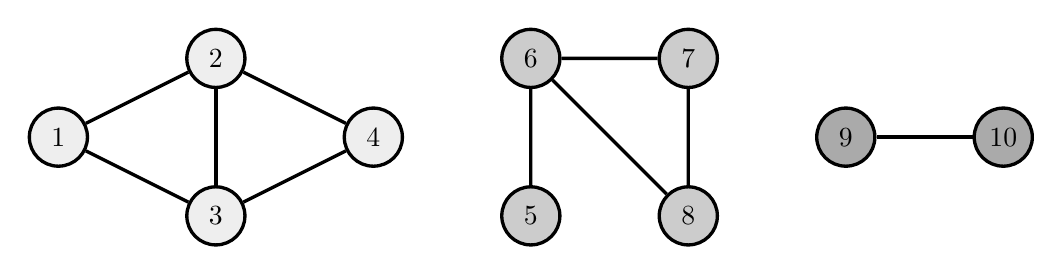
\begin{tikzpicture}[very thick,level/.style={sibling distance=70mm/#1}]
\draw (0, 0) node [vertex] (n1) {1};
\draw (2, 1) node [vertex] (n2) {2};
\draw (2, -1) node  [vertex] (n3) {3};
\draw (4, 0) node [vertex] (n4) {4};
\draw (n1) -- (n2);
\draw (n2) -- (n3);
\draw (n3) -- (n4);
\draw (n2) -- (n4);
\draw (n1) -- (n3);
\draw (6, -1) node [vertex, fill=mysalmon] (n5) {5};
\draw (6, 1) node [vertex, fill=mysalmon] (n6) {6};
\draw (8, 1) node [vertex, fill=mysalmon] (n7) {7};
\draw (8, -1) node [vertex, fill=mysalmon] (n8) {8};
\draw (n5) -- (n6) -- (n7) -- (n8) -- (n6);
\draw (10, 0) node[vertex, fill=mypurple] (n9) {9};
\draw (12, 0) node[vertex, fill=mypurple] (n10) {10};
\draw (n9) -- (n10);
\end{tikzpicture}
\caption{This diagram illustrates a graph with three connected components. \textit{Credit: Samuel Hsiang}}
\end{figure}

Determining which components are connected can be done with DFS/BFS in $O(V+E)$ time. Pick a vertex that has not been visited, mark it with unique identifier and as visited, and recur on all connected neighbors, marking them with the same identifier. Continue this process until all vertices have been visited.

\subsection{Dynamic Connectivity}
\textit{Dynamic connectivity} is an extension of connectivity. We want to be able to add edges and merge components, but also determine if two vertices are in the same component at any time. For the purpose of this lecture, we will not consider removing edges. 

Specifically, we want to support the following operations.

\begin{itemize}
    \item $find(v):$ Determine which component $v$ is in.
    \item $union(u, v): $ Connect vertices $u$ and $v$.
\end{itemize}

\section{Union Find (Disjoint Set Union)}
The goal of the \textit{union find data structure}, aka \textit{disjoint set data structure} is to solve these queries efficiently. We discuss two approaches:

\begin{itemize}
    \item \textit{Quick Find}: Represent the problem with an array. Every index represents a vertex and holds the component id. This performs \textit{find} in $O(1)$ (index lookup) and \textit{union} in $O(N)$ (iterate through the entire array to change the elements). This is equivalent to running flood fill for every union operation.
    \item \textit{Quick Union}: For each node, we can maintain a parent pointer to one other node that it’s connected to. Eventually, following these pointers will lead to a root node that points to itself. Since all nodes in the component point to it, it is the \textit{representative element} of the component. This forms a collection of trees, also known as a \texit{forest}.
\end{itemize}

\pagebreak

\begin{figure}[h]
\centering
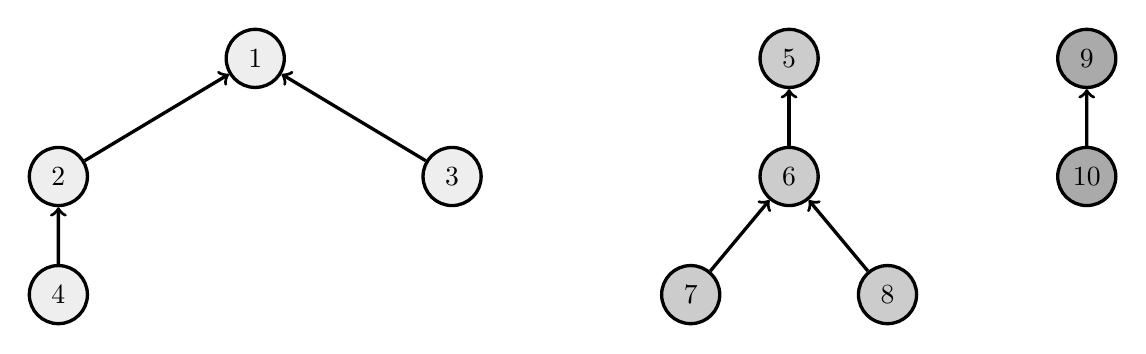
\begin{tikzpicture}[very thick,edge from parent/.style={draw,<-},level/.style={sibling distance=50mm/#1}]
\node [vertex, fill = mysalmon] (r2) {5}
  child {
      node [vertex, fill = mysalmon] {6}
      child { node [vertex, fill=mysalmon] {7} }
      child { node [vertex, fill=mysalmon] {8} }
  };

\node [vertex] [left=6cm of r2] (r1) {1}
  child {
    node [vertex] {2}
    child {
      node [vertex] {4}
    }
  }
  child {node [vertex] {3} };
  
\node [vertex, fill=mypurple] [right=3cm of r2] (r3) {9}
  child { node [vertex, fill=mypurple] {10} };
\end{tikzpicture}
\caption{Representation of union-find as a forest. \textit{Credit: Samuel Hsiang}}
\end{figure}

\section{Quick Union}
With quick-find, we update every element in one connected component whenever we perform a union, which requires
us to search the entire array. Instead, \textit{quick union} takes a lazier approach and only updates the pointer of the root element.
This takes advantage of the interpretation of union-find as a tree.

\begin{itemize}
    \item \textit{find(v):} Follow the parent pointer of $v$ until we reach the root and return root id.
    \item \textit{union(u, v):} Change the parent pointer of $find(u)$ to point to $find(v)$.
\end{itemize}
\\
If we number our nodes sequentially, we can represent the pointers as an array.

\begin{figure}[h]
\centering
{
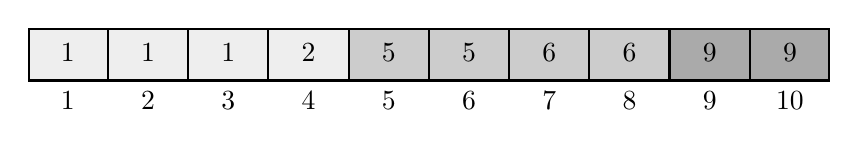
\begin{tikzpicture}[
  thick,
  myrect/.style={
    draw,
    rectangle split,
    rectangle split horizontal,
    rectangle split parts=#1,
    rectangle split part align=left,
    text width=5ex,
    text centered
    },
  mycallout/.style={
    shape=rectangle callout,
    rounded corners,
    fill=mysalmon,
    callout absolute pointer={#1},
    callout pointer width=1cm
  }  
]

\node[myrect=10, rectangle split part fill={myseagreen, myseagreen, myseagreen, myseagreen, mysalmon, mysalmon, mysalmon, mysalmon, mypurple, mypurple}]
  (array1)
  {
  					\strut 1
  \nodepart{two}	\strut 1
  \nodepart{three}	\strut 1
  \nodepart{four}	\strut 2
  \nodepart{five}	\strut 5
  \nodepart{six}	\strut 5
  \nodepart{seven}	\strut 6
  \nodepart{eight}	\strut 6
  \nodepart{nine}	\strut 9
  \nodepart{ten}	\strut 9
  };
\foreach \Valor [count=\Valori from 1] in {one ,two ,three ,four ,five ,six ,seven ,eight ,nine ,ten }
  \node[below] at (array1.\Valor south) {\Valori};

\end{tikzpicture}
}
\caption{Pointer Array.
\textit{Credit: Samuel Hsiang}}
\end{figure}

Because \textit{find} traverses the tree until it reaches a root element, its worst-case complexity is $O(N)$, proportional to the height of the tree. And because \textit{union} requires us to call \textit{find}, its complexity is also $O(N)$. This is worse than Quick-find! But we can significantly improve \textit{find} by limiting the depth of the tree.

\subsection{Weighting}
Whenever we perform \textit{union}, if we keep track of the size of each tree, we can always join a smaller tree to the root of a larger tree, rather than the other way around. This optimization limits the maximum depth of any tree to $\log N$. This means that the cost of both \textit{find} and \textit{union} are now $O(\log N)$.

\subsection{Path compression}
Intuitively, flattening the tree would make the find operation faster by shortening the number of pointers we need to traverse. So another optimization we can make is every time we perform $find(v)$, to change $v$ and all of its parents to point to its root node. This allows us to avoid traversing the same path more than once.

Combining weighting with path compression brings down the cost of \textit{find} and \textit{union} to amortized $O(\alpha(N))$, where $\alpha$ represents the extremely slowly-growing \textit{inverse Ackermann function}. For practical purposes, $\alpha(N)<5$. In fact, this is asymptotically optimal: union-find in constant time is impossible.

\pagebreak

\section{Pseudocode}
This is a sample implementation of weighted quick-union with path compression. \textit{Credit: Samuel Hsiang}

\begin{algorithm}[H]
\caption{Union-Find}
%\label{}
\begin{algorithmic}
\Function{Find}{$v$}
	\If {$parent(v)$ is v}
		\State \Return $v$
    \EndIf
    \State $parent(v) \gets \Call{Find}{parent(v)}$
    \State \Return $parent(v)$
\EndFunction
\Function{Union}{$u$, $v$}
	\State $uRoot \gets \Call{Find}{u}$
	\State $vRoot \gets \Call{Find}{v}$
    \If {$uRoot = vRoot$}
		\State \Return
	\EndIf
    \If {$size(uRoot)<size(vRoot)$}
    	\State $parent(uRoot) \gets vRoot$
        \State $size(vRoot) \gets size(uRoot) + size(vRoot)$
    \Else
    	\State $parent(vRoot) \gets uRoot$
        \State $size(uRoot) \gets size(uRoot) + size(vRoot)$
    \EndIf
\EndFunction
\end{algorithmic}
\end{algorithm}

\section{Minimum Spanning Trees}
Consider a \textit{connected}, \textit{undirected} graph. A \textit{spanning tree} is a subgraph that is a tree and contains every vertex in the original graph. A \textit{minimum spanning tree} is a spanning tree such that the sum of the edge weights of the tree is minimized. 

\begin{figure}[!htbp]
\centering
{
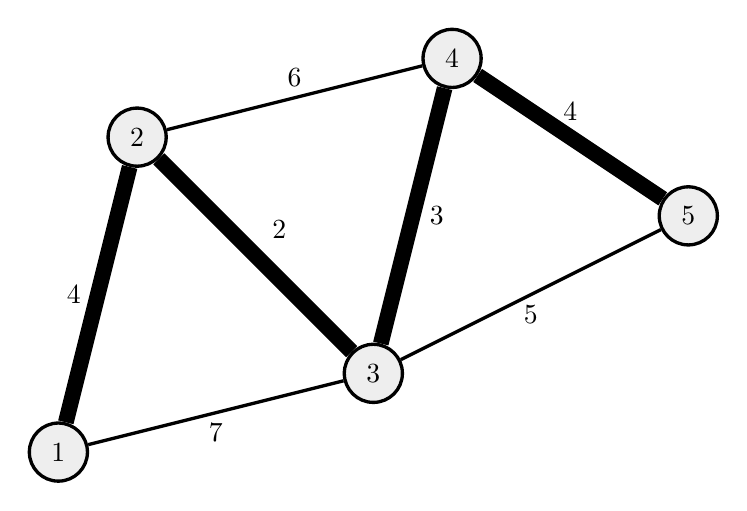
\begin{tikzpicture}[very thick,edge from parent/.style={draw,<-},level/.style={sibling distance=30mm/#1}]
\draw (0, 0) node [vertex] (v1) {1};
\draw (1, 4) node [vertex] (v2) {2};
\draw (4, 1) node [vertex] (v3) {3};
\draw (5, 5) node [vertex] (v4) {4};
\draw (8, 3) node [vertex] (v5) {5};
\draw[line width=2mm] (v1) -- (v2) node[midway, left] {4};
\draw[line width=2mm] (v2) -- (v3) node[midway, above right] {2};
\draw (v1) -- (v3) node[midway, below] {7};
\draw (v2) -- (v4) node[midway, above] {6};
\draw[line width=2mm] (v3) -- (v4) node[midway, right] {3};
\draw (v3) -- (v5) node[midway, below] {5};
\draw[line width=2mm] (v4) -- (v5) node[midway, above] {4};
\end{tikzpicture}
}
\caption{Figure 4: MST.
\textit{Credit: Samuel Hsiang}}
\end{figure}

\subsection{Kruskal's Algorithm}
We begin with every node being its own disjoint set. We construct a MST by greedily adding edges from lowest to highest weight. However, a tree is defined as having no cycles (cannot leave a node from an edge and enter through a different edge), so if two nodes are already in the same component, we disregard that edge. The MST of $n$ nodes always contains exactly $n-1$ edges, so we can stop looking through more edges after adding $n-1$ edges to the MST. Conveniently, union find works perfectly for this. This algorithm requires sorting the edges and thus has complexity $O(ElogE + E\alpha(V))$. 

\begin{algorithm}[H]
\caption{Kruskal}
\begin{algorithmic}
\ForAll{edges $(u,v)$ in sorted order}
	\If{$\Call{Find}{u} \not= \Call{Find}{v}$}
		\State add $(u,v)$ to spanning tree
		\State $\Call{Union}{u,v}$
	\EndIf
\EndFor
\end{algorithmic}
\end{algorithm}

\subsection{Example}
Moocast (USACO Gold, December 2016) \\ \\
Farmer John's Cows ($1 \leq N \leq 1000$) each have a walkie talkie. They will spend $X$ dollars such that each walkie talkie has transmission radius $\sqrt{N}$. Each cow can communicate another as the cows can relay their message through some sequence of transmissions. Determine the minimum cost such that every cow can communicate with another.

\subsection{Example 2}
Superbull (USACO Silver, February 2015) \\ \\
Given $N\leq2000$ teams and the "excitement" caused by a match between every pair of teams, find the most excitement possible in a tournament.  The loser is eliminated after every game, but you get to pick who loses.

\section{Monotonic Queries}
You are given a graph and a set of chronological queries (by time, value, etc) that ask about the state of the components at that given state.

All we have to do maintain the state of the components using union find over the chronology. In fact, this is exactly how we build MSTs (state is weight of edge, query is do we have one component given we follow the rules for MSTs?).    

\subsection{Offline Queries}
What if they are not in order? If all you need to do is read the queries and answer them within the time limit, it is an easy extension to monotonic queries. Store the initial order of the queries, sort the queries, and answer them like monotonic queries. Each answer is mapped to its respective query. Then, loop through the initial order, extracting the respective stored answers.  

\subsection{Example}
Mootube (USACO Gold, January 2018) \\ \\
Farmer John created Mootube, where every two connected videos have a relevance value. He wants to filter content using this metric. Specifically, given a value $k$ and the video the user is currently watching, connected videos are suggested to a user if their relevance is greater than $k$. Moreover, this process is recursive, meaning if a third video not directly connected to the first is relevant to some chain of relevant videos, it is also relevant. 

Given $1 \leq Q \leq 100000$ queries, each with two values, $v$, $k$, representing the current video and metric used, how many relevant videos are there?

\end{document}
